%This is the introduction...
%
%\vspace{0.5cm}
%
%\begin{figure}[]
%  \centering
%  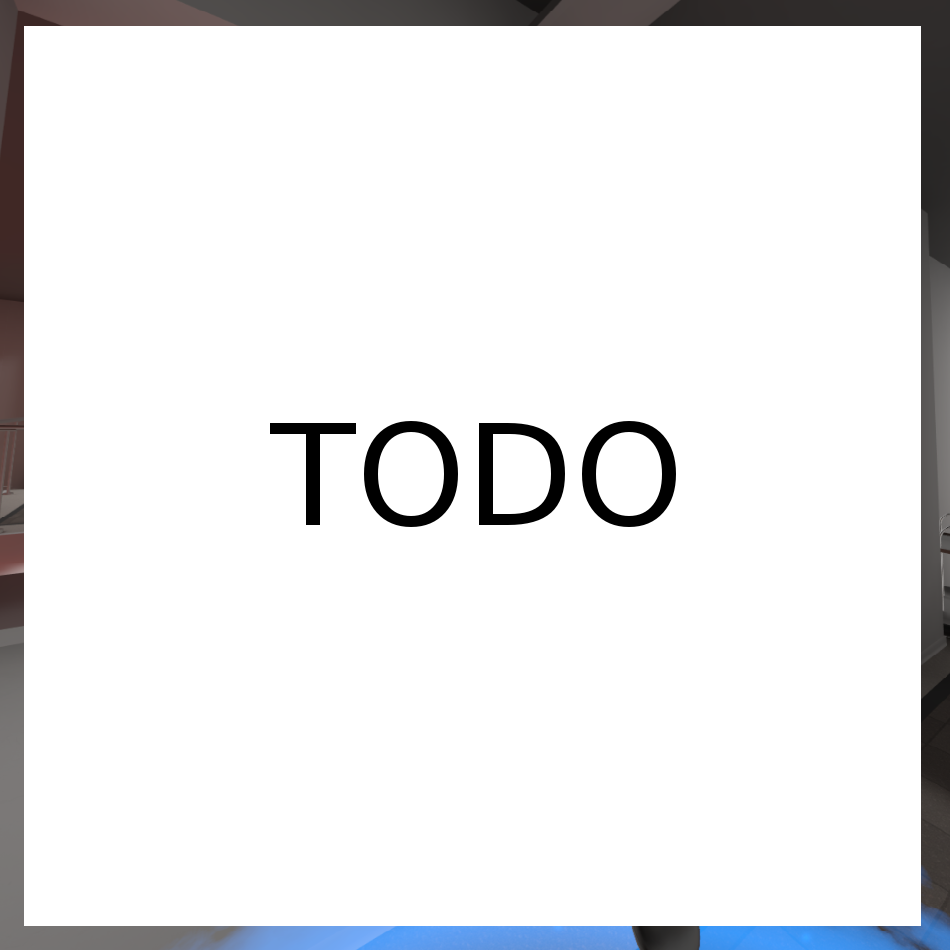
\includegraphics[width=0.5\textwidth]{images/todo.png}
%  \caption{This is an example ToDo picture.}
%  \label{fig:todo}
%\end{figure}
%
%Hypotheses and sub-hypotheses can be formulated like this:
%
%\begin{hypothesis}
%\label{hyp:test}
%This is a hypothesis.
%\end{hypothesis}
%
%\begin{shypothesis}
%\label{shyp:test}
%This is a sub-hypothesis.
%\end{shypothesis}
%
%Hypothesis \cref{hyp:test} is very importance and must be referenced in the text.
\label{Chapter:Introduction}
Many navigation techniques exist for both Desktop and Immersive \acrfull{ve} that define how users moves around these \acrshort{ve}s. The goals of navigation are to move towards a target location and orientation to explore the environment. Navigation should facilitate way finding in the \acrshort{ve}, which means allowing the user to know where they are, where they will go next and how they will get there. This also means that the user should have a good perception of the \acrshort{ve} and path that they took. Navigation techniques have to ensure that there is minimal motion sickness, sufficient environmental awareness which means that while navigating the user knows where they are in an environment compared to where they were before and that it is easy to reach important places in the environment. Two common metaphors for navigation are steering and teleportation.

Steering navigation is a technique where there is continuous movement in a direction indicated either by gaze, pointing or use of a physical device. In some cases an additional action can be added to specify the velocity. With steering navigation spatial awareness is generally good but can cause motion sickness. Teleportation navigation is a target based metaphor for where the goal position is specified discretely by pointing or choosing a location and orientation to be moved towards. This form of navigation minimises motion sickness but results in less environmental awareness as compared to the steering metaphor. Some techniques try to reconcile these two metaphors to minimise motion sickness while still maintaining a good environmental awareness. One example is the jumping metaphor presented by Weissker et al. which \textit{'only allows to teleport to locations in the currently visible part of the scene'} which makes it a short range version of the teleportation metaphor~\cite{Weissker2018}. 

Navigation techniques can be active such that the user is controlling their own movement; passive such that the user is being automatically moved around the environment; or they can be a mix of active and passive. Navigation techniques can also provide the user with guidance regardless of whether this is active or passive. Guided navigation techniques such as the river analogy presented by Galyean, which guides \textit{'the user’s continuous and direct input within both space and time allowing a more narrative presentation'} and uses automatic steering for guided navigation allow for the addition of a narrative structure to a \acrshort{ve}~\cite{Galyean1995}. In this work we will explore guided navigation using the jumping metaphor instead of a steering one and investigate the benefits of an automatic approach over a user controlled one for a museum setting. 

This thesis will discuss work related to navigation techniques and guiding in \acrshort{ve}s on \acrfull{hmd}s in Chapter \ref{chapter:Related Work}. 
